% Created 2022-11-09 Wed 09:23
% Intended LaTeX compiler: pdflatex
\documentclass[10pt]{beamer}
\usepackage[utf8]{inputenc}
\usepackage[T1]{fontenc}
\usepackage{graphicx}
\usepackage{longtable}
\usepackage{wrapfig}
\usepackage{rotating}
\usepackage[normalem]{ulem}
\usepackage{amsmath}
\usepackage{amssymb}
\usepackage{capt-of}
\usepackage{hyperref}
\usepackage{minted}
\usepackage[T1]{fontenc}
\usepackage{pmboxdraw}
\usetheme{Berkeley}
\usefonttheme{professionalfonts}
\usepackage{booktabs}
\definecolor{mycolor}{rgb}{0.54706, 0.13725, 0.26667}
\usecolortheme[named=mycolor]{structure}
\setlength{\parskip}{5pt}
\newcommand{\footnoteframe}[1]{\footnote[frame]{#1}}
\addtobeamertemplate{footnote}{}{\vspace{2ex}}
\usepackage{xcolor}
\definecolor{LightGray}{gray}{0.95}
\setbeamertemplate{caption}[numbered]
\usepackage{amsmath}
\usepackage{fancyvrb}
\DefineVerbatimEnvironment{verbatim}{Verbatim}{fontsize=\scriptsize}
\DeclareGraphicsRule{.gif}{png}{-0.png}{`convert #1 `dirname #1`/`basename #1 .gif`-gif-converted-to.png}
\DeclareGraphicsExtensions{.gif}
\usepackage{animate}
\usetheme{default}
\author{Jay Morgan}
\date{9th October 2022}
\title{Machine Learning}
\subtitle{Lecture 1 - Introductions}
\hypersetup{
 pdfauthor={Jay Morgan},
 pdftitle={Machine Learning},
 pdfkeywords={},
 pdfsubject={},
 pdfcreator={Emacs 28.1 (Org mode 9.5.5)}, 
 pdflang={English}}
\begin{document}

\maketitle

\section*{Introduction}
\label{sec:orgac4a82f}

\subsection*{Course Organisation}
\label{sec:orgab771b7}

\begin{frame}[label={sec:org5dff354}]{Welcome!}
Welcome to all the new students! Here I am going to be talking about Machine Learning
and all of the great things that this "technology" has to offer. To begin our course,
I shall start with a bit of house keeping -- more specifically, I will be talking
about what exactly we'll be learning about in the course (Machine Learning is a broad
subject after-all). In addition, I will tell you where you can find the resources
related to the course and how you can contact me, should you have any questions.
\end{frame}

\begin{frame}[label={sec:orgaf4f4e4}]{What this course is about?}
In this course, we will be learning about Machine Learning: firstly, what Machine
Learning actually is; secondly, we'll take a look at some of the algorithms within
the scope of Machine Learning, and develop an intuition about how these algorithms
work and when they would be useful; and finally, how we can compare and evaluate the
algorithms we've learnt about.
\end{frame}

\begin{frame}[label={sec:org626e08f}]{How this course will be taught}
I intended to deliver this course via a series of lectures. These lectures will be
accompanied by the PDF lecture slides, in which I will provide the definitions and
provide reference links should you wish to do some extra reading.
\end{frame}

\begin{frame}[label={sec:org3e1bbdd}]{Outline of the course}
\begin{center}
\begin{tabular}{rlll}
\toprule
Lecture & Expected date & Type & Topic\\
\midrule
1 & 9th November & Theory & Introduction\\
2 & 16th November & Theory & Linear models\\
3 & 22nd November & Lab & Lab on Linear models\\
4 & 25th November & Theory/Lab & Evaluation of models\\
5 & 29th November & Theory/Lab & Support Vector Machines\\
6 & 2nd December & Theory/Lab & Kernel methods\\
\bottomrule
\end{tabular}
\end{center}
\end{frame}

\subsection*{Reading the lectures}
\label{sec:org7d7c318}

\begin{frame}[label={sec:org7a9f785},fragile]{Source code}
 During the course, I would also like to supplement my algorithmic definitions and
explanations with some programming code -- for this I will use the \href{https://www.python.org/}{Python} programming
language. The code snippets would look something like:

\begin{minted}[frame=lines,linenos=true,firstnumber=last,fontsize=\footnotesize,bgcolor=LightGray,xleftmargin=5pt,tabsize=2,breaklines=true,numbersep=10pt]{python}
import random
x = [1, 2, 3, 4]
y = [random.random() + xi for xi in x]
print(y)
\end{minted}

\begin{verbatim}
[1.4898241502582414, 2.4805286156642175, 3.065379052563245, 4.05328483072365]
\end{verbatim}
\end{frame}

\begin{frame}[label={sec:orgb042edd},fragile]{Running the source code yourself}
 All of the source can be run by yourselves if you use the same python environment
(i.e. that you have installed all the appropriate libraries). On the git repository,
I've included the \href{https://git.sr.ht/\~jaymorgan/teaching/tree/master/item/2022-2023/Machine\%20Learning/environment.yml}{\texttt{environment.yml}} file used in the production of these lectures.

To run the code:

\begin{minted}[frame=lines,linenos=true,firstnumber=last,fontsize=\footnotesize,bgcolor=LightGray,xleftmargin=5pt,tabsize=2,breaklines=true,numbersep=10pt]{bash}
wget https://git.sr.ht/~jaymorgan/teaching/blob/master/2022-2023/Machine%20Learning/environment.yml
conda env create -f environment.yml  # recreate the conda env
conda activate ml-lectures           # activate the new env
python <scripts>
\end{minted}
\end{frame}

\begin{frame}[label={sec:org4a063c3}]{References}
In some cases, and is the norm with academic traditions, we'll want to include a
reference, a link to previous written works.

Here is an example of a sentence that includes a reference:

"This is a very important sentence which I assert to be true, to convince you of this
fact I shall appeal to authority and include a reference:
(Shalev-Shwartz, Shai and Ben-David, Shai, 2014)"

More information on the referenced material (such as title, publishing date) will be
found in the bibliography slide (or bottom of the webpage if you're viewing the HTML
version of the lectures).
\end{frame}

\begin{frame}[label={sec:org4a47783}]{About Me}
My name is Dr Jay Morgan. I am a researcher at the Université de Toulon, where I am
developing Deep Learning models (a sub-field of Machine Learning research) for the
study of astrophysical phenomenon.

You can find more information and links on my personal (LIS-Lab) website:
\url{https://pageperso.lis-lab.fr/jay.morgan/}

I also publish libraries and source code online:
\begin{itemize}
\item Github: \url{https://github.com/jaypmorgan}
\item Gitlab: \url{https://gitlab.com/jaymorgan}
\item Source Hut: \url{https://sr.ht/\~jaymorgan/}
\end{itemize}

If you have any questions, you can email me at jay.morgan@univ-tln.fr
\end{frame}

\begin{frame}[label={sec:org8d7e189}]{Where you can find the resources}
I try to make this course as accessible as possible, which means that I host these
slides in a variety of ways to suit you.

Firstly, you can find the links to all my courses on my personal website at:
\url{https://pageperso.lis-lab.fr/jay.morgan/teaching.html}

Here you can find the links to each lecture in a PDF or HTML format. Additionally,
you can view the source code used to make these lectures on source hut:
\url{https://git.sr.ht/\~jaymorgan/teaching}. On this git repository you can find all my
lectures from all years.
\end{frame}

\section*{What is learning, anyway?}
\label{sec:org8e90b9f}

\subsection*{Learning about Learning}
\label{sec:org90bae5c}

\begin{frame}[label={sec:orge687f7c}]{Let's answer the question of learning}
We'll begin our journey into the world of Machine Learning by tackling the question
of what it means to 'learn' -- how may a machine actually \emph{learn} anything?
\end{frame}

\begin{frame}[label={sec:orgf62d368}]{Bait-shyness}
\begin{center}

\includegraphics[height=0.7\textheight]{images/rat.jpg}
\end{center}

To begin to answer the question of learning, we may turn to nature for
advice. Principally, if we look at the studies conducted with Mice we find some idea
to notion of learning (Shalev-Shwartz, Shai and Ben-David, Shai, 2014). (Image by brgfx on Freepik)

When a rat encounters a novel source of food, it will first eat a little bit of
it. If the food is edible for the rat, it will continue to eat the food, even in
future encounters. If, however, on the initial contact with the food, the rat deems
the food poisonous, it will ignore and not eat the food in future encounters. This
process we call 'bait-shyness'.

Here then we see the rat, on finding something new, learn from its experience, and
use that knowledge of the experience for future encounters.

Our initial understanding of rat's bait-shyness was limited, but we've come to
understand more about it. For instance, we learn that their learning process is more
complex than originally thought. In a later experiment, where the 'poison' in the
food is replaced by a different unpleasant stimulus such as a electric shock --
i.e. when a rat eats a food, it is then shocked. It was found that this did not
deter the rat from eating the food in future encounters, unlike the poison.

It is presumed that the rat's have some 'prior knowledge' about the world and do not
infer a temporal relationship between the food and being shocked, while they can
infer the same relationship with food and illness.
\end{frame}

\begin{frame}[label={sec:orgd5ed126}]{Computer Programs}
From these two examples of how rats may learn we see: the rat will make a guess about
something new (i.e. that the food is not poisonous), it will find out how good this
guess is (i.e. it either gets ill or it does not), and learn from how well its guess
was for the future. We also see that its learning can be impacted by the rat's prior
knowledge about how the world may work.

But how does this \emph{framework} for the process of learning translate to computers? For a
more formal definition of how computer programs could be said to learn, we have a
similar idea:

\begin{quote}
A computer program is said to learn from experience \(E\) with respect
to some class of tasks \(T\) and performance measure \(P\), if its performance
a tasks in \(T\), as measured by \(P\), improves with experience \(E\).
\end{quote}

(Mitchell, Tom M, 1997)
\end{frame}

\begin{frame}[label={sec:orga3066b9},fragile]{Quiz!}
 What \emph{function} is being used here?

\begin{verbatim}
8 ? 5   =   13
9 ? 1   =   10
1 ? 2   =    3
\end{verbatim}
\end{frame}

\begin{frame}[label={sec:orga53b68d},fragile]{Something more difficult\ldots{}}
 What \emph{values} are being used here?

\begin{verbatim}
x * 1 + y   =   4
x * 3 + y   =   8
x * 5 + y   =  12
\end{verbatim}
\end{frame}

\begin{frame}[label={sec:org70e4b51}]{When might we need Machine Learning}
\begin{center}
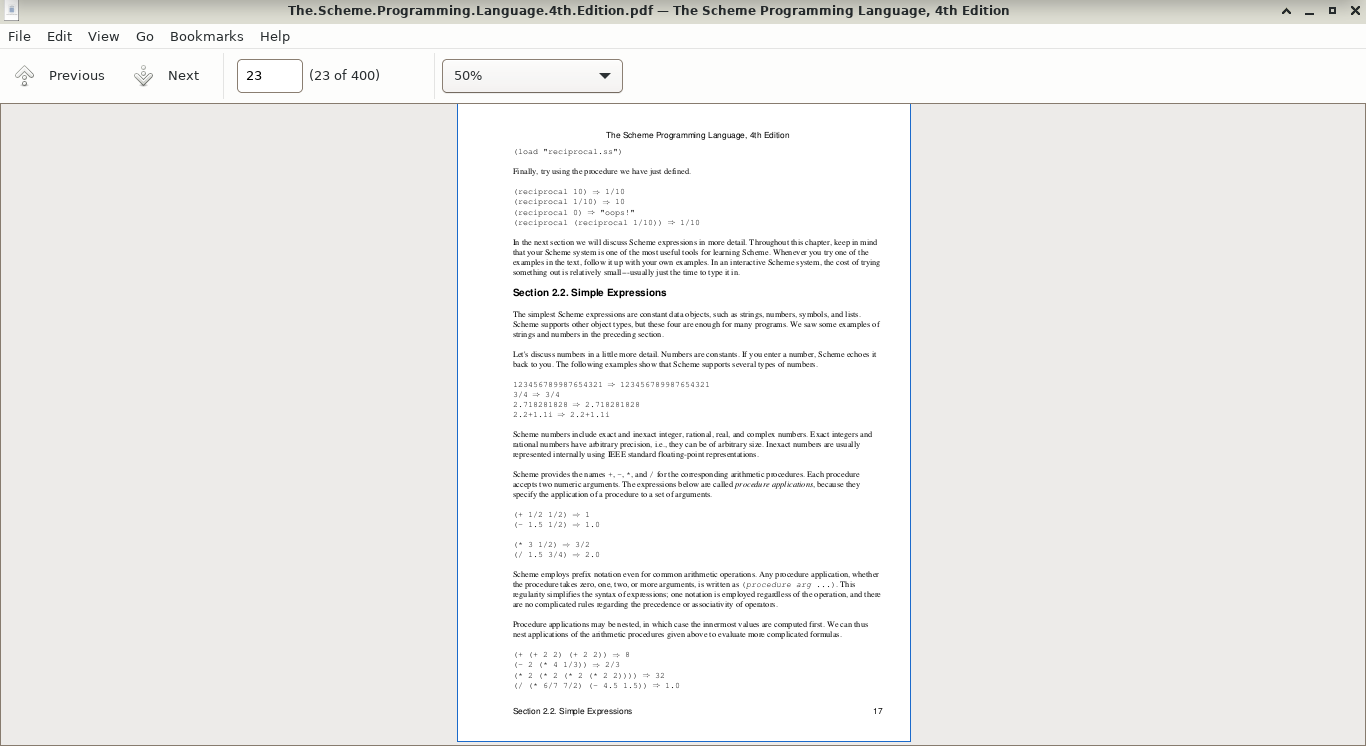
\includegraphics[height=0.7\textheight]{images/pdf-ocr.png}
\end{center}

Why do we need computer programs that 'learn' anyway? We already have programming
languages, why can't we just use them?

Let's suppose we're creating a very simple Optical Character Recognition (OCR)
program.

This program looks at a PDF document and converts the text into something we
can copy and paste. Part of this program's task is to take an individual character,
say the number '8', and recognise that it's an 8 and add that to the already scanned
text.

How would we go about creating a program where we can define how to identify '8' or
'1' or 'l' -- with all the varieties of lighting conditions, handwriting, fonts,
sizes. We could find the process of encompassing all different variations tiresome --
if not impossible, and that's only for a single character!
\end{frame}

\begin{frame}[label={sec:org30909dd}]{When might we need Machine Learning}
With Machine Learning, instead of enumerating all possible solutions within a
programming language, we collect a bunch of examples of '8's and give them to the
algorithm to learn from.

Through looking at these many different examples, the algorithm will/should be able
to recognise what an 8 generally looks like.
\end{frame}

\begin{frame}[label={sec:orgb265e49}]{Different types of Learning}
What we have just demonstrated by way of the OCR example, is the type of learning we
call 'Supervised Learning'. We have many examples of input (lots of different kinds
of handwritten 8's), and we tell the learning algorithm, that they are indeed the
number 8.

But there are other kind of different learning frameworks. Specifically we have the
following:

\begin{itemize}
\item Supervised Learning
\item Unsupervised, or sometimes called self-supervised Learning
\item Reinforcement Learning
\end{itemize}
\end{frame}

\begin{frame}[label={sec:org29aee83}]{Supervised Learning}
To better formalise Supervised Learning from our previous OCR example, Supervised
Learning is when the learning algorithm "see's" or has access to both the input and
output.

Let's have a dataset \(X\), which is a set consisting of tuple pairs \(x_i, y_i\). \(x_i\)
is an input, i.e. a single image with an '8', and \(y_i\) is a label which tells the
learning algorithm if the input is indeed an '8' or something else. Mathematically we have:

\(X = \{(x_1, y_1), (x_2, y_2), ..., (x_n, y_n)\}\)
\end{frame}

\begin{frame}[label={sec:orgcc94bab}]{Unsupervised Learning}
In Unsupervised learning, we have again have a dataset \(X\), who's elements are only
inputs. In other words, there are no corresponding labels for each input. Instead,
the learning algorithm must learn inherent patterns in the data and create labels
itself. Throughout the course, we'll see examples of Unsupervised Learning in action.

One thing to note: Recent methodologies have started to call Unsupervised Learning,
self-supervised. As we have just discussed, the labels are inherent to the data from
the discovered patterns, it's just we are not explicitly giving them to the learning
algorithm ourselves. So it's sort of like a supervised learning setup, except the
learning algorithm is providing the labels itself -- hence the self-supervised.
\end{frame}

\begin{frame}[label={sec:org7bbda04}]{Reinforcement Learning}
Reinforcement Learning is very different to both Supervised and Unsupervised
Learning. Here is the type of learning you might be familiar with if you've seen 'AI'
that learns to play video games. In this type of learning, we have the following
elements:

\begin{itemize}
\item An agent
\item An environment
\item A set of allowed actions the agent can make within its environment.
\end{itemize}

In this situation, an agent will interact with it's environment, and when it does
something it can receive a reward (a reward can be positive or negative). The agent
will remember what it has done to receive the reward. The objective for the agent is
to maximise the reward score, and learns to do this through many iterations or
play-through.
\end{frame}

\subsection*{Terminology}
\label{sec:orgb6bb86e}

\begin{frame}[label={sec:orgf13e762}]{What will our data look like?}
In this section we shall take a look at the different types of data we might expect
and the different terminology used to name them.

Data in Machine Learning applications can come in a variety of different formats. The
most typical data formats we might see are:

\begin{itemize}
\item Tables
\item Images/Videos
\item Text
\item Sound
\end{itemize}

These are the initial formats, though, before actually doing any learning, we will
want to transform them into a different representation that we can use.
\end{frame}

\begin{frame}[label={sec:org3afcc97}]{Tables}
A table, or tabular, format is a \(n \times m\) set of data with \(n\) samples or
examples, and \(m\) features for each sample. For example, suppose we have a table
consisting the price of 100 different houses:

\begin{center}
\begin{tabular}{rrll}
\toprule
Number of bedrooms & Garden size (ft) & \ldots{} & Price (\$)\\
\midrule
3 & 0 & \ldots{} & 150,000\\
5 & 10 & \ldots{} & 200,000\\
\ldots{} & \ldots{} & \ldots{} & \\
10 & 1000 & \ldots{} & 2,000,000\\
\bottomrule
\end{tabular}
\end{center}

In a supervised learning setting, where we want to predict the price of a house we may then have the following dataset:

\(X = \{([3, 0, ...], 150,000), ([5, 10, ...], 200,000), \\..., ([10, 1000, ...], 2,000,000)\}\)
\end{frame}

\begin{frame}[label={sec:org6838791}]{Images/Videos}
Images are composed of 2D or 3D arrays of numeric values. For example, in a RGB
image that is 1024x500 pixels, we would have the array of size 1024x500x3 -- where 3
is the red, green, and blue channel, respectively. If we have just a grayscale image,
we could represent it as either 1024x500x1 or 1024x500 as the channel 'dimension' of
the array is singular.

We may already know that videos are simply a sequence of images that are iterated
through 24+ times a second. For a 24 frames per second video, we would have an array
size of 1024x500x3x24 -- a 4-dimensional array.
\end{frame}

\begin{frame}[label={sec:orgbaecb3b}]{Text}
Text and language data is perhaps one of the most flexible formats of data, in terms
of the person implementing the Machine Learning algorithm is somewhat free in
determining how to represent the language to the algorithm.

With text data, we have a series of 'tokens' -- these tokens could be words, groups
of words, parts of words, and even just characters. For example, consider:

"this is a sentence, that shouldn't be misunderstood."
\end{frame}

\begin{frame}[label={sec:org572d26f}]{Tokenisation of text}
"this is a sentence, that shouldn't be misunderstood."

We could 'tokenise' (the process of converting a string into a series of tokens that
represent the original string) this sentence by splitting at white-space:

\(\{"this", "is", "a", "sentence,", "that" "shouldn't", "be", "misunderstood."\}\)

Notice how with the words "sentence" and "misunderstood", the punctuation is
considered part of the word and so "misunderstood." != "misunderstood".

These kinds of questions of how to best represent text and language we will talk more
about in later lectures!
\end{frame}

\begin{frame}[label={sec:org9d809f8}]{Time-series}
I named this section time-series to be as general as possible. Within the type
'time-series', we could have the following types of information:

\begin{itemize}
\item Sound waves
\item Stock prices
\item Network messaging
\end{itemize}

These types of data all share a property in that the 'time' component is important in
their meaning.  
\end{frame}

\subsection*{Example Problems}
\label{sec:org25fda99}

\begin{frame}[label={sec:org3a03fc3}]{Example Problems}
Throughout this course, we'll be using \emph{toy} datasets for the explanation of Machine
Learning and its algorithms. In this section, we'll take a broad look over all the
datasets that we'll come to be very familiar with.
\end{frame}

\begin{frame}[label={sec:orge15805c}]{Types of Outputs -- Regression \& Classification}
First, however, I wish to explain the difference between the terms \emph{Regression} and
\emph{Classification}.

\begin{itemize}
\item Regression: the prediction of a continuous quantity, i.e. how much does this house cost?
\item Classification: the prediction of a discrete value or class label, i.e. dog or cat?
\end{itemize}

In the following toy datasets, we'll see different types of predictions that fall
under the regression/classification output type.
\end{frame}

\begin{frame}[label={sec:org27182e4}]{Boston House Prices Dataset -- Tabular Regression}
A dataset of 506 houses in Boston, USA, collected during US Census.

\begin{itemize}
\item 13 features/properties about each house
\item 1 target property: the price of the house
\end{itemize}

More information about each of the features can be found at: \url{https://www.cs.toronto.edu/\~delve/data/boston/bostonDetail.html}

(Harrison Jr, David and Rubinfeld, Daniel L, 1978)
\end{frame}

\begin{frame}[label={sec:org31db6e5},fragile]{Boston House Prices -- example rows}
 \begin{minted}[frame=lines,linenos=true,firstnumber=last,fontsize=\footnotesize,bgcolor=LightGray,xleftmargin=5pt,tabsize=2,breaklines=true,numbersep=10pt]{python}
import warnings
from sklearn.datasets import load_boston
with warnings.catch_warnings():
    warnings.filterwarnings("ignore")
    boston = load_boston()
boston = pd.DataFrame(
    data=np.c_[boston['data'], boston['target']],
    columns=boston['feature_names'].tolist() + ['target'])
print(boston[:2])
\end{minted}

\begin{verbatim}
      CRIM    ZN  INDUS  CHAS    NOX     RM  ...  RAD    TAX  PTRATIO      B  LSTAT  target
0  0.00632  18.0   2.31   0.0  0.538  6.575  ...  1.0  296.0     15.3  396.9   4.98    24.0
1  0.02731   0.0   7.07   0.0  0.469  6.421  ...  2.0  242.0     17.8  396.9   9.14    21.6

[2 rows x 14 columns]
\end{verbatim}
\end{frame}

\begin{frame}[label={sec:orgc4cf7b4}]{Boston House Prices -- concerns}
The Boston dataset is an excellent dataset in the fact that it contains some ethical
issues when it comes to Machine Learning. More specifically, some of the features in
the data are 'dummy' variables for racial attributes (Carlisle, M., 2020). Moreover, these features show a
racial segregation has a positive impact on house prices.

Scikit-Learn (scikit-learn, 2022), one of the most prolific Machine Learning framework in the Python
ecosystem, has decided to depreciate and remove the Boston dataset from their
repository following these concerns.

We will continue to use the dataset here as it is an easy to understand regression
problem, and to demonstrate how easy it is to be accidentally unethical if you're not
thinking about the data carefully enough. 
\end{frame}

\begin{frame}[label={sec:orgf4fa726}]{Iris Dataset -- Tabular Classification}
\begin{figure}[htbp]
\centering
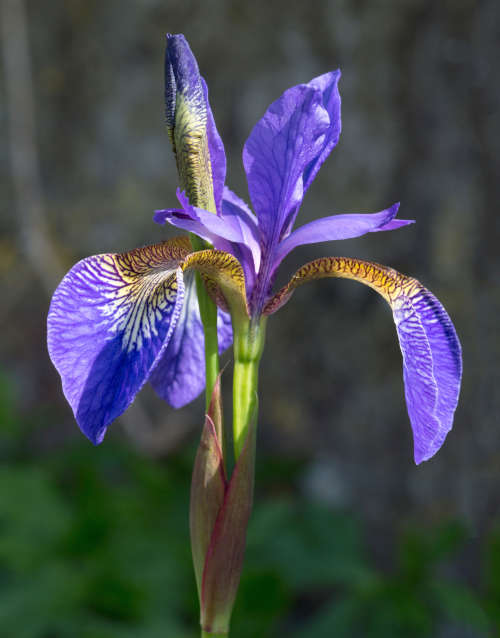
\includegraphics[width=0.4\textwidth]{images/iris.jpg}
\caption{Iris Flower (Diliff, 2014)}
\end{figure}
\end{frame}

\begin{frame}[label={sec:org0226960}]{Iris Dataset -- features}
\begin{columns}
\begin{column}{0.5\columnwidth}
\begin{itemize}
\item 150 examples
\item 4 features: Petal length/width, sepal length/width
\item 1 classification: type of flower: \{virginica, setosa, veriscolor\}

\url{https://archive.ics.uci.edu/ml/datasets/iris}
(Fisher, Ronald A, 1936)
\end{itemize}
\end{column}

\begin{column}{0.4\columnwidth}
\begin{figure}[htbp]
\centering
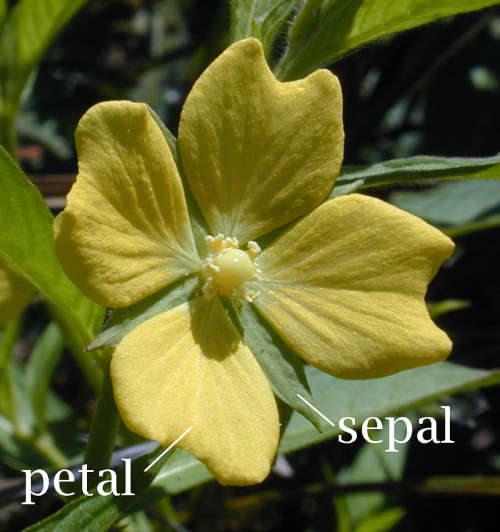
\includegraphics[width=0.8\textwidth]{images/Petal-sepal.jpg}
\caption{Different parts of a flower. (Eric Guinther, 2005)}
\end{figure}
\end{column}
\end{columns}
\end{frame}

\begin{frame}[label={sec:orge0118b0},fragile]{Iris Dataset -- example rows}
 \begin{minted}[frame=lines,linenos=true,firstnumber=last,fontsize=\footnotesize,bgcolor=LightGray,xleftmargin=5pt,tabsize=2,breaklines=true,numbersep=10pt]{python}
from sklearn.datasets import load_iris
iris = load_iris()
iris = pd.DataFrame(
    data = np.c_[iris['data'], iris['target']],
    columns = iris['feature_names'] + ['target'])
print(iris.head(2))
\end{minted}

\begin{verbatim}
   sepal length (cm)  sepal width (cm)  petal length (cm)  petal width (cm)  target
0                5.1               3.5                1.4               0.2     0.0
1                4.9               3.0                1.4               0.2     0.0
\end{verbatim}
\end{frame}

\begin{frame}[label={sec:org46dd72b}]{MNIST Dataset -- Image Classification}
\begin{figure}[htbp]
\centering
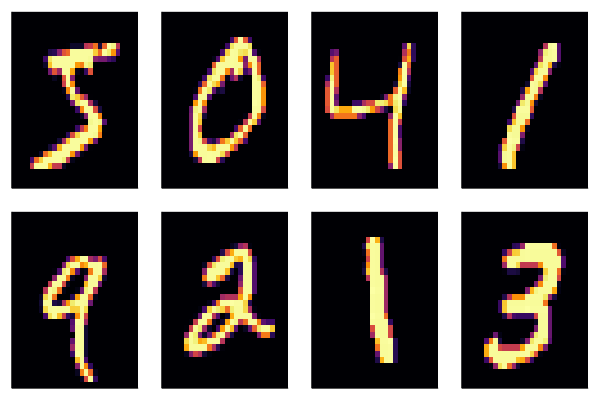
\includegraphics[width=0.5\textwidth]{images/mnist.png}
\caption{8 examples of handwritten digits in the MNIST dataset.}
\end{figure}

A dataset of images (of size 28x28) containing handwritten digits from 0 - 9.

\url{http://yann.lecun.com/exdb/mnist/}

(LeCun, Yann and Bottou, L{\'e}on and Bengio, Yoshua and Haffner, Patrick, 1998)
\end{frame}

\begin{frame}[label={sec:org20d38b9}]{MNIST Dataset -- Features}
\begin{itemize}
\item 60,000 images in the training dataset
\item 10,000 images in the test dataset
\item 28x28 pixels (grayscale)
\end{itemize}
\end{frame}

\begin{frame}[label={sec:org1d34594},fragile]{MNIST Dataset -- Example Rows}
 \begin{minted}[frame=lines,linenos=true,firstnumber=last,fontsize=\footnotesize,bgcolor=LightGray,xleftmargin=5pt,tabsize=2,breaklines=true,numbersep=10pt]{python}
from sklearn.datasets import fetch_openml
mnist = fetch_openml("mnist_784").data[:2]
\end{minted}
\end{frame}

\begin{frame}[label={sec:orgb853a8c},fragile]{Large Movie Review Dataset -- Text Classification/Regression}
 \begin{verbatim}
Story of a man who has unnatural feelings for a pig. Starts out with a
opening scene that is a terrific example of absurd comedy. A formal
orchestra audience is turned into an insane, violent mob by the crazy
chantings of it's singers. Unfortunately it stays absurd the WHOLE
time with no general narrative eventually making it just too off
putting. Even those from the era should be turned off. The cryptic
dialogue would make Shakespeare seem easy to a third grader. On a
technical level it's better than you might think with some good
cinematography by future great Vilmos Zsigmond. Future stars Sally
Kirkland and Frederic Forrest can be seen briefly.
\end{verbatim}

Review from: \texttt{train/neg/0\_3.txt}

\begin{itemize}
\item 50,000 movie reviews (25,000 for training and testing).
\item Each review is labelled with a binary label of sentiment -- a positive or negative
review was towards the movie in question.
\end{itemize}

\url{https://ai.stanford.edu/\~amaas/data/sentiment/}

(Maas, Andrew L. and Daly, Raymond E. and Pham, Peter T. and Huang, Dan and Ng, Andrew Y. and Potts, Christopher, 2011)
\end{frame}

\begin{frame}[fragile,allowframebreaks,label=]{Ham or Spam -- Text Classification}
 \begin{verbatim}
Message-ID: <8701134.1075856113926.JavaMail.evans@thyme>
Date: Mon, 30 Oct 2000 02:06:00 -0800 (PST)
From: shona.wilson@enron.com
To: eugenio.perez@enron.com
Subject: meeting deadlines
Mime-Version: 1.0
Content-Type: text/plain; charset=us-ascii
Content-Transfer-Encoding: 7bit
X-From: Shona Wilson
X-To: Eugenio Perez
X-cc: 
X-bcc: 
X-Origin: Beck-S
X-FileName: sbeck.nsf

Dear Eugenio,

I did not want to say this when everyone else was around, but I am concerned 
that no attempt was made to meet the deadline of this morning that we 
discussed last Friday. (to decide on a name for the database).  Only Maria 
Teresa had her information to me this am as requested. The deadline could 
have been easily met by working diligently this morning, but Jennifer did not 
come in until 8:30 and MT until 8:15.

I thought we had discussed the urgency of this - to have something to present 
at the 10am meeting.  We need to discuss this to ensure it does not happen 
again.

Best regards

Shona
\end{verbatim}

\begin{itemize}
\item Enron Spam classification of email messages.
\item Is the email Spam -- each email is labelled with a binary label, spam or not spam
(ham).
\item The dataset contains 17,171 spam and 16,545 ham email messages.
\end{itemize}

\url{https://www2.aueb.gr/users/ion/data/enron-spam/}

(Metsis, Vangelis and Androutsopoulos, Ion and Paliouras, Georgios, 2006)
\end{frame}

\subsection*{Concerns \& Considerations}
\label{sec:org011f4f5}

\begin{frame}[label={sec:orgef70fef}]{Concerns \& Considerations}
As we saw with the Boston house prices dataset, ethical concerns can easily arise
when we use statistical analysis \& Machine Learning. But our use of Machine Learning
carries many more concerns other than just racial biases. In this section, we'll
highlight some ethical considerations to be made when designing and building Machine
Learning models.

\url{https://uksa.statisticsauthority.gov.uk/publication/ethical-considerations-in-the-use-of-machine-learning-for-research-and-statistics/}
\end{frame}

\begin{frame}[label={sec:orgdd96dd5}]{Compute resources -- environmental concerns}
\begin{quote}
Large-scale deployment of AI could also have both positive and negative impacts on
the environment. Negative impacts include increased use of natural resources, such as
rare earth metals, pollution and waste, as well as energy consumption. However, AI
could help with waste management and conservation offering environmental benefits.
\end{quote}

\begin{quote}
[\ldots{}] In the United States, data centres already account for about 2 percent of all
electricity used. In one estimation, DeepMind's AlphaGo – which beat Go Champion Lee
Sedol in 2016 – took 50,000 times as much power as the human brain to do so.
\end{quote}

({European Parliament. Directorate General for Parliamentary Research Services.}, 2020)
\end{frame}

\begin{frame}[label={sec:orga260e42}]{Bias in language models}
\begin{figure}[htbp]
\centering
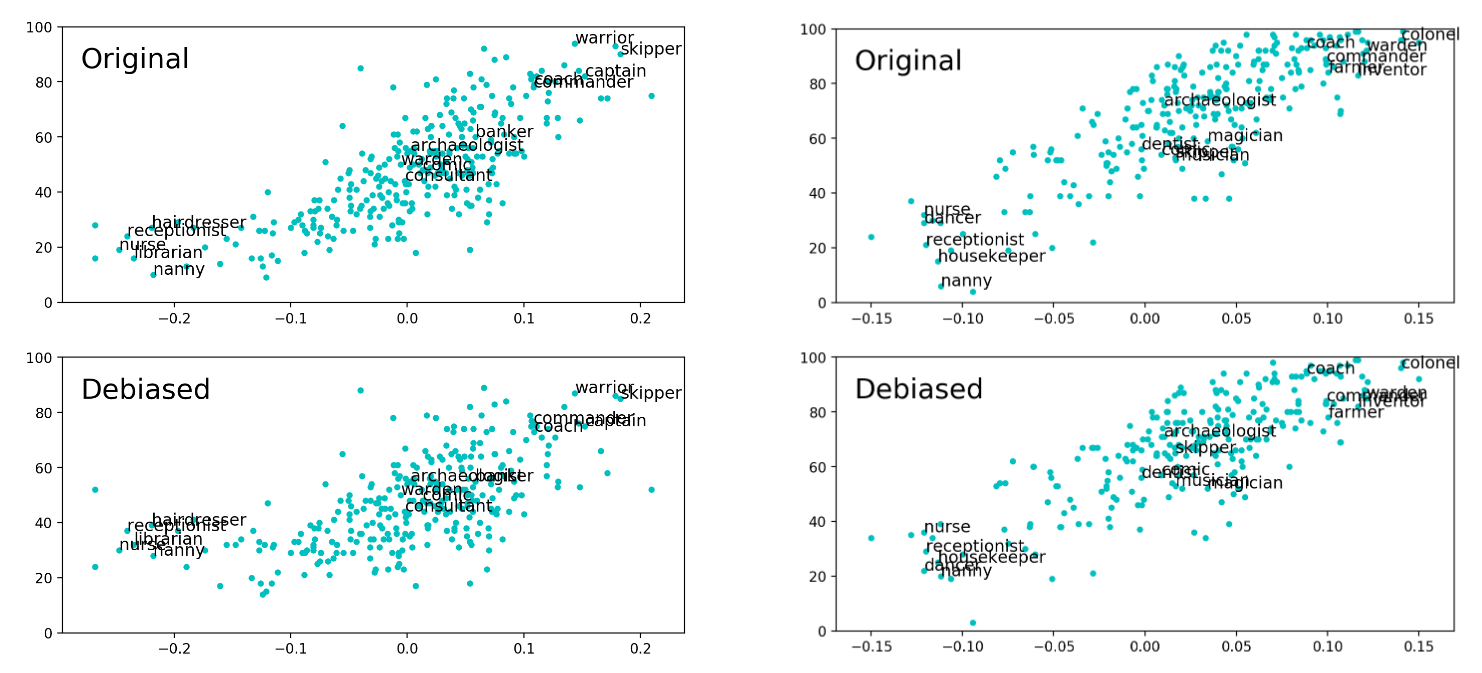
\includegraphics[width=1.0\textwidth]{images/debias.png}
\caption{(Gonen, Hila and Goldberg, Yoav, 2019)}
\end{figure}

Biases exist in language models trained on news articles (Bolukbasi, Tolga and Chang, Kai-Wei and Zou, James Y and Saligrama, Venkatesh and Kalai, Adam T, 2016).
\end{frame}

\begin{frame}[label={sec:org545298e}]{Personal information}
In Machine Learning applications where data is generated (such as generating faces
that don't exist), there is a possibility to expose personal information. For
example, in a situation where these generative Machine Learning models create
synthetic patient data, the model may be trained on real medical data. The output of
the Machine Learning model could possibly leak personal information.

(Arora, Anmol and Arora, Ananya, 2022)
\end{frame}

\begin{frame}[label={sec:orgcbf7227}]{Mental health of optimisation algorithms}
This example is more specific to how algorithms are used as opposed to their specific
design. Yet, this should still be highlighted. We have seen increasing discussion
surrounding the use of optimisation algorithms that try to increase the amount of
'screen time' or engagement from users of social media, and it's no secret that
spending lots of time of social media has a measurable effect on one's mental health.
\end{frame}

\begin{frame}[fragile,allowframebreaks,label=]{Copyright Concerns}
 A more recent addition to the concerns is that of Github's co-pilot application that
helps users write programming code. This application has been developed on
open-source software -- some of which includes licensing that specifies how this
open-source code may be used (for example, with attribution or copy-left). Yet,
Github's co-pilot may insert code that its been trained on verbatim (though recent
additions have been addressing these concerns), resulting in a situation of 'code
laundering'. \url{https://twitter.com/mitsuhiko/status/1410886329924194309}

\begin{minted}[frame=lines,linenos=true,firstnumber=last,fontsize=\footnotesize,bgcolor=LightGray,xleftmargin=5pt,tabsize=2,breaklines=true,numbersep=10pt]{c}
float Q_rsqrt( float number )
{
        long i;
        float x2, y;
        const float threehalfs = 1.5F;

        x2 = number * 0.5F;
        y  = number;
        i  = * ( long * ) &y;                       // evil floating point bit level hacking
        i  = 0x5f3759df - ( i >> 1 );               // what the fuck? 
        y  = * ( float * ) &i;
        y  = y * ( threehalfs - ( x2 * y * y ) );   // 1st iteration
//	y  = y * ( threehalfs - ( x2 * y * y ) );   // 2nd iteration, this can be removed

        return y;
}

// Implementation from Quake III Arena under the GPL license.
\end{minted}
\end{frame}

\section*{Summary}
\label{sec:org224648d}

\begin{frame}[label={sec:org12b11a7}]{What is Machine Learning}
\begin{itemize}
\item We've taken a look at the different kinds of frameworks for learning -- animal
behaviour with bait-shyness, and how that translates in computer programs.
\item We've identified the different types of learning: supervised, unsupervised, and
reinforcement learning.
\item We've looked at the different types of data we may encounter, from tabular to text
data, and have also seen examples of some toy datasets we will be using in the course.
\item Finally, we've highlighted some of the ethical concerns that can arise in Machine
Learning.
\end{itemize}
\end{frame}

\section*{Bibliography}
\label{sec:org35f4e83}

\begin{frame}[fragile,allowframebreaks,label=]{Bibliography}
\noindent
Arora, Anmol and Arora, Ananya (2022). \emph{Generative Adversarial Networks and Synthetic Patient Data: Current Challenges and Future Perspectives}, {Royal College of Physicians}.

\noindent
Bolukbasi, Tolga and Chang, Kai-Wei and Zou, James Y and Saligrama, Venkatesh and Kalai, Adam T (2016). \emph{Man is to computer programmer as woman is to homemaker? debiasing word embeddings}, Advances in neural information processing systems.

\noindent
Carlisle, M. (2020). \emph{Racist Data Destruction?}, Medium.

\noindent
Diliff (2014). \emph{Iris germanica (Purple bearded Iris), Wakehurst Place, UK - Diliff.jpg}.

\noindent
Eric Guinther (2005). \emph{Image of a primrose willowherb Ludwigia octovalvis (family Onagraceae), flower showing petals and sepals}.

\noindent
{European Parliament. Directorate General for Parliamentary Research Services.} (2020). \emph{The Ethics of Artificial Intelligence: Issues and Initiatives.}, {Publications Office}.

\noindent
Fisher, Ronald A (1936). \emph{The use of multiple measurements in taxonomic problems}, Wiley Online Library.

\noindent
Gonen, Hila and Goldberg, Yoav (2019). \emph{Lipstick on a {{Pig}}: {{Debiasing Methods Cover}} up {{Systematic Gender Biases}} in {{Word Embeddings But}} Do Not {{Remove Them}}}, {arXiv}.

\noindent
Harrison Jr, David and Rubinfeld, Daniel L (1978). \emph{Hedonic housing prices and the demand for clean air}, Elsevier.

\noindent
LeCun, Yann and Bottou, L{\'e}on and Bengio, Yoshua and Haffner, Patrick (1998). \emph{Gradient-based learning applied to document recognition}, Ieee.

\noindent
Maas, Andrew L. and Daly, Raymond E. and Pham, Peter T. and Huang, Dan and Ng, Andrew Y. and Potts, Christopher (2011). \emph{Learning Word Vectors for Sentiment Analysis}, Association for Computational Linguistics.

\noindent
Metsis, Vangelis and Androutsopoulos, Ion and Paliouras, Georgios (2006). \emph{Spam filtering with naive bayes-which naive bayes?}.

\noindent
Mitchell, Tom M (1997). \emph{Machine learning}, McGraw-hill New York.

\noindent
scikit-learn (2022). \emph{Sklearn.Datasets.Load\_boston}, scikit-learn.

\noindent
Shalev-Shwartz, Shai and Ben-David, Shai (2014). \emph{Understanding machine learning: From theory to algorithms}, Cambridge university press.
\end{frame}
\end{document}
